% 4.静电场习题解答.tex
\section{静电场习题解答}

\begin{enumerate}[label=\arabic*.]
% 第1题
\item 在直角坐标系中，已知电场强度 \(\vec{E} = 6x^2\vec{e}_x + 6y\vec{e}_y + 4\vec{e}_z\ \text{V/m}\)，点 \(M\) 和 \(N\) 的坐标分别为点 \(M(2,6,-1)\)、点 \(N(-3,-3,2)\)，试求：
\begin{enumerate}
    \item \(\varphi_{MN} = ?\)；
    \item 若点 \(Q(4,-2,-35)\) 为参考点，则 \(\varphi_M = ?\)；
    \item 若点 \(P(1,2,-4)\) 处的电位为 2V，则 \(\varphi_N = ?\)
\end{enumerate}

\textbf{解答：}

首先求\textbf{电位函数} \(\varphi(x,y,z)\)。
由 \(\vec{E} = -\nabla\varphi\)，可得：
\[
\begin{cases}
E_x = -\dfrac{\partial \varphi}{\partial x} = 6x^2 \\
E_y = -\dfrac{\partial \varphi}{\partial y} = 6y \\
E_z = -\dfrac{\partial \varphi}{\partial z} = 4
\end{cases}
\]

分别积分得：
\[
\varphi(x,y,z) = -2x^3 - 3y^2 - 4z + C
\]
其中 \(C\) 为积分常数，由\textbf{电位参考点}条件决定。

\vspace{0.5em}
(1) 两点间\textbf{电位差}：
\[
\varphi_{MN} = \varphi_M - \varphi_N
\]

计算 \(\varphi_M\) 和 \(\varphi_N\)：
\[
\varphi_M = -2(2)^3 - 3(6)^2 - 4(-1) + C = -16 - 108 + 4 + C = -120 + C
\]
\[
\varphi_N = -2(-3)^3 - 3(-3)^2 - 4(2) + C = 54 - 27 - 8 + C = 19 + C
\]

因此：
\[
\varphi_{MN} = (-120 + C) - (19 + C) = -139\ \text{V}
\]

\vspace{0.5em}
(2) 以点 \(Q(4,-2,-35)\) 为参考点，即 \(\varphi_Q = 0\)：
\[
\varphi_Q = -2(4)^3 - 3(-2)^2 - 4(-35) + C = -128 - 12 + 140 + C = 0 \implies C=0
\]

电位函数为 \(\varphi(x,y,z) = -2x^3 - 3y^2 - 4z\)。
则 \(M\) 点电位：
\[
\varphi_M = -2(2)^3 - 3(6)^2 - 4(-1) = -16 - 108 + 4 = -120\ \text{V}
\]

\vspace{0.5em}
(3) 已知点 \(P(1,2,-4)\) 处电位为 2V：
\[
\varphi_P = -2(1)^3 - 3(2)^2 - 4(-4) + C = -2 - 12 + 16 + C = 2 + C = 2\ \text{V}
\]

解得 \(C=0\)。
则 \(N\) 点电位：
\[
\varphi_N = -2(-3)^3 - 3(-3)^2 - 4(2) = 54 - 27 - 8 = 19\ \text{V}
\]

\vspace{1em}

% 第2题
\item 在直角坐标系中电荷分布为 \(\rho(x,y,z)\)，试求电场强度 \(\vec{E}\)，其中
\[
\rho(x,y,z) =
\begin{cases}
\rho_0, & x = 0 \\
0, & x \neq 0
\end{cases}
\]

\textbf{解答：}

题目中电荷仅分布在 \(x=0\) 平面上，属于\textbf{面电荷分布}，其\textbf{面电荷密度}为：
\[
\rho_s = \rho_0 \quad (\text{单位：C/m}^2)
\]

根据对称性，电场强度 \(\vec{E}\) 只有 \(x\) 方向分量，且与 \(y,z\) 无关。利用\textbf{高斯定理}求解：

取高斯面为跨接在 \(x=0\) 平面两侧的柱形闭合面，柱体轴线沿 \(x\) 轴，端面垂直于 \(x\) 轴，面积为 \(A\)。

由高斯定理：
\[
\oint_S \vec{E} \cdot d\vec{S} = \frac{Q_{\text{enc}}}{\varepsilon_0}
\]
其中闭合面内包围电荷 \(Q_{\text{enc}} = \rho_s A = \rho_0 A\)。

\begin{itemize}
    \item 对于 \(x>0\) 区域：电场方向沿 \(+\vec{e}_x\)，\(E_x = E\)
    \item 对于 \(x<0\) 区域：电场方向沿 \(-\vec{e}_x\)，\(E_x = -E\)
\end{itemize}

高斯面通量仅由两个端面贡献：
\[
\oint_S \vec{E} \cdot d\vec{S} = E \cdot A + E \cdot A = 2EA
\]

代入高斯定理：
\[
2EA = \frac{\rho_0 A}{\varepsilon_0} \implies E = \frac{\rho_0}{2\varepsilon_0}
\]

因此，电场强度为：
\[
\vec{E}(x) =
\begin{cases}
\dfrac{\rho_0}{2\varepsilon_0} \vec{e}_x, & x > 0 \\
-\dfrac{\rho_0}{2\varepsilon_0} \vec{e}_x, & x < 0
\end{cases}
\]

\vspace{1em}

% 第3题
\item 对于下面给出的几种 \(\vec{D}\) 场，试求相应的\textbf{体电荷密度}表达式：
\begin{enumerate}
    \item \(\displaystyle \vec{D} = \frac{4xy}{z}\vec{e}_x + \frac{2x^2}{z}\vec{e}_y - \frac{2x^2y}{z^2}\vec{e}_z\)；
    \item \(\displaystyle \vec{D} = z\sin\phi\vec{e}_\rho + z\cos\phi\vec{e}_\phi + \rho\sin\phi\vec{e}_z\)
\end{enumerate}

\textbf{解答：}

根据介质中高斯定理微分形式，自由体电荷密度 \(\rho_f = \nabla \cdot \vec{D}\)。

\vspace{0.5em}
(1) 直角坐标系下的\textbf{散度}：
\[
\nabla \cdot \vec{D} = \frac{\partial D_x}{\partial x} + \frac{\partial D_y}{\partial y} + \frac{\partial D_z}{\partial z}
\]

分别求偏导：
\[
\frac{\partial D_x}{\partial x} = \frac{\partial}{\partial x}\left( \frac{4xy}{z} \right) = \frac{4y}{z}
\]
\[
\frac{\partial D_y}{\partial y} = \frac{\partial}{\partial y}\left( \frac{2x^2}{z} \right) = 0
\]
\[
\frac{\partial D_z}{\partial z} = \frac{\partial}{\partial z}\left( -\frac{2x^2y}{z^2} \right) = \frac{4x^2y}{z^3}
\]

因此：
\[
\rho_f = \frac{4y}{z} + \frac{4x^2y}{z^3} = \frac{4y}{z}\left( 1 + \frac{x^2}{z^2} \right)
\]

\vspace{0.5em}
(2) 柱坐标系下的散度：
\[
\nabla \cdot \vec{D} = \frac{1}{\rho}\frac{\partial (\rho D_\rho)}{\partial \rho} + \frac{1}{\rho}\frac{\partial D_\phi}{\partial \phi} + \frac{\partial D_z}{\partial z}
\]

分别求偏导：
\[
\frac{1}{\rho}\frac{\partial (\rho D_\rho)}{\partial \rho} = \frac{1}{\rho}\frac{\partial}{\partial \rho}\left( \rho \cdot z\sin\phi \right) = \frac{z\sin\phi}{\rho}
\]
\[
\frac{1}{\rho}\frac{\partial D_\phi}{\partial \phi} = \frac{1}{\rho}\frac{\partial}{\partial \phi}\left( z\cos\phi \right) = -\frac{z\sin\phi}{\rho}
\]
\[
\frac{\partial D_z}{\partial z} = \frac{\partial}{\partial z}\left( \rho\sin\phi \right) = 0
\]

因此：
\[
\rho_f = \frac{z\sin\phi}{\rho} - \frac{z\sin\phi}{\rho} + 0 = 0
\]

\vspace{1em}

% 第4题
\item 在空间区域为 \(x=0\) 到 \(1\)，\(y=0\) 到 \(2\)，\(z=0\) 到 \(3\) 的平行六面体内，有矢量场 \(\vec{D} = 2xy\vec{e}_x + x^2\vec{e}_y\ \text{C/m}^2\)。试计算平行六面体内的\textbf{总电荷量}。

\textbf{解答：}

根据高斯定理，闭合曲面内的总电荷量等于电位移矢量的体积分：
\[
Q = \iiint_V \rho_f \, dV = \iiint_V (\nabla \cdot \vec{D}) \, dV
\]

首先计算体电荷密度 \(\rho_f = \nabla \cdot \vec{D}\)：
\[
\nabla \cdot \vec{D} = \frac{\partial D_x}{\partial x} + \frac{\partial D_y}{\partial y} + \frac{\partial D_z}{\partial z}
\]

其中：
\[
D_x = 2xy, \quad D_y = x^2, \quad D_z = 0
\]

因此：
\[
\frac{\partial D_x}{\partial x} = 2y, \quad \frac{\partial D_y}{\partial y} = 0, \quad \frac{\partial D_z}{\partial z} = 0
\]

所以：
\[
\rho_f = 2y
\]

对 \(\rho_f\) 在平行六面体内积分，求总电荷量：
\[
Q = \int_{x=0}^{1} \int_{y=0}^{2} \int_{z=0}^{3} 2y \, dz \, dy \, dx
\]

分步计算：
\begin{enumerate}
    \item 对 \(z\) 积分：
    \[
    \int_{z=0}^{3} dz = 3
    \]
    \item 对 \(y\) 积分：
    \[
    \int_{y=0}^{2} 2y \cdot 3 \, dy = 3 \int_{0}^{2} 2y \, dy = 3 \left[ y^2 \right]_0^2 = 12
    \]
    \item 对 \(x\) 积分：
    \[
    Q = \int_{x=0}^{1} 12 \, dx = 12
    \]
\end{enumerate}

因此，平行六面体内的总电荷量为 \(Q = 12\ \text{C}\)。

\vspace{1em}

% 第5题
\item 无限长同轴圆柱面，半径分别为 \(a\) 和 \(b\)（\(b > a\)），每单位长度上电荷：内柱上为 \(\tau\)，外柱为 \(-\tau\)。求真空中带电面之间的\textbf{电压}。

\textbf{解答：}

根据电荷分布的轴对称性，两圆柱面之间（\(a < \rho < b\)）的电场强度可由高斯定理求得。

取半径为 \(\rho\)、长度为 \(l\) 的同轴圆柱面为高斯面，由高斯定理：
\[
\oint_S \vec{E} \cdot d\vec{S} = \frac{Q_{\text{enc}}}{\varepsilon_0}
\]

高斯面内包围的电荷为 \(Q_{\text{enc}} = \tau l\)，电场仅沿径向 \(\vec{e}_\rho\) 方向，因此：
\[
E \cdot 2\pi\rho l = \frac{\tau l}{\varepsilon_0}
\]

解得：
\[
E(\rho) = \frac{\tau}{2\pi\varepsilon_0 \rho} \quad (a < \rho < b)
\]

两圆柱面之间的电压（电位差）为：
\[
U_{ab} = \varphi_a - \varphi_b = \int_{a}^{b} \vec{E} \cdot d\vec{\rho}
\]

代入电场表达式：
\[
U_{ab} = \int_{a}^{b} \frac{\tau}{2\pi\varepsilon_0 \rho} d\rho = \frac{\tau}{2\pi\varepsilon_0} \ln \frac{b}{a}
\]

因此，两圆柱面之间的电压为：
\[
U = \frac{\tau}{2\pi\varepsilon_0} \ln \frac{b}{a}
\]

\vspace{1em}

% 第6题
\item 从静电场基本性质出发，证明当电介质均匀时，\textbf{极化电荷密度} \(\rho_p\) 存在的条件是自由电荷的体密度 \(\rho\) 不为零，且有关系式
\[
\rho_p = -\left(1 - \frac{\varepsilon_0}{\varepsilon}\right)\rho
\]

\textbf{证明：}

1. 根据介质中的高斯定理微分形式：
\[
\nabla \cdot \vec{D} = \rho
\]
其中电位移矢量 \(\vec{D} = \varepsilon \vec{E}\)（均匀线性介质），代入得：
\[
\nabla \cdot (\varepsilon \vec{E}) = \rho
\]

由于介质均匀，\(\varepsilon\) 为常数，可提出散度外：
\[
\varepsilon \nabla \cdot \vec{E} = \rho \implies \nabla \cdot \vec{E} = \frac{\rho}{\varepsilon}
\]

\vspace{0.5em}
2. 同时，电场强度的散度满足：
\[
\nabla \cdot \vec{E} = \frac{\rho + \rho_p}{\varepsilon_0}
\]
其中 \(\rho_p\) 为极化电荷体密度。

\vspace{0.5em}
3. 联立上述两式：
\[
\frac{\rho}{\varepsilon} = \frac{\rho + \rho_p}{\varepsilon_0}
\]

交叉相乘并整理：
\[
\rho \varepsilon_0 = \varepsilon(\rho + \rho_p)
\]
\[
\varepsilon \rho_p = \rho \varepsilon_0 - \varepsilon \rho
\]
\[
\rho_p = \rho \left( \frac{\varepsilon_0}{\varepsilon} - 1 \right) = -\left(1 - \frac{\varepsilon_0}{\varepsilon}\right)\rho
\]

\vspace{0.5em}
4. 结论：
\begin{itemize}
    \item 若 \(\rho = 0\)，则 \(\rho_p = 0\)，即均匀介质内部无自由电荷时，也无极化体电荷；
    \item 只有当 \(\rho \neq 0\) 时，\(\rho_p\) 才不为零，且满足 \(\rho_p = -\left(1 - \frac{\varepsilon_0}{\varepsilon}\right)\rho\)。
\end{itemize}

\vspace{1em}

% 第7题
\item 已知真空中有三个点电荷 \(q_1 = 1\,\text{C}\)，\(q_2 = 1\,\text{C}\)，\(q_3 = 4\,\text{C}\)，分别位于 \((1,0,0)\)、\((0,1,0)\)、\((-1,0,0)\) 点，求 \((1,1,1)\) 点的\textbf{电场强度}。

\textbf{解答：}

点电荷的电场强度公式为：
\[
\vec{E} = \frac{1}{4\pi\varepsilon_0} \frac{q}{|\vec{r} - \vec{r}'|^3} (\vec{r} - \vec{r}')
\]
其中 \(\vec{r}=(1,1,1)\) 为场点，\(\vec{r}'\) 为源点。

\vspace{0.5em}
1. 计算 \(q_1\) 在 \((1,1,1)\) 点的电场 \(\vec{E}_1\)
\[
\vec{r} - \vec{r}_1' = (0,1,1),\quad |\vec{r} - \vec{r}_1'| = \sqrt{2}
\]
\[
\vec{E}_1 = \frac{1}{4\pi\varepsilon_0} \frac{1}{2\sqrt{2}} (0,1,1)
\]

\vspace{0.5em}
2. 计算 \(q_2\) 在 \((1,1,1)\) 点的电场 \(\vec{E}_2\)
\[
\vec{r} - \vec{r}_2' = (1,0,1),\quad |\vec{r} - \vec{r}_2'| = \sqrt{2}
\]
\[
\vec{E}_2 = \frac{1}{4\pi\varepsilon_0} \frac{1}{2\sqrt{2}} (1,0,1)
\]

\vspace{0.5em}
3. 计算 \(q_3\) 在 \((1,1,1)\) 点的电场 \(\vec{E}_3\)
\[
\vec{r} - \vec{r}_3' = (2,1,1),\quad |\vec{r} - \vec{r}_3'| = \sqrt{6}
\]
\[
\vec{E}_3 = \frac{1}{4\pi\varepsilon_0} \frac{4}{6\sqrt{6}} (2,1,1) = \frac{1}{4\pi\varepsilon_0} \frac{2}{3\sqrt{6}} (2,1,1)
\]

\vspace{0.5em}
4. 总电场强度叠加 \(\vec{E} = \vec{E}_1 + \vec{E}_2 + \vec{E}_3\)
\[
E_x = \frac{1}{4\pi\varepsilon_0} \left( 0 + \frac{1}{2\sqrt{2}} + \frac{4}{3\sqrt{6}} \right)
\]
\[
E_y = \frac{1}{4\pi\varepsilon_0} \left( \frac{1}{2\sqrt{2}} + 0 + \frac{2}{3\sqrt{6}} \right)
\]
\[
E_z = \frac{1}{4\pi\varepsilon_0} \left( \frac{1}{\sqrt{2}} + \frac{2}{3\sqrt{6}} \right)
\]

整理可得：
\[
\vec{E} = \frac{1}{4\pi\varepsilon_0} \left[
\left( \frac{1}{2\sqrt{2}} + \frac{4}{3\sqrt{6}} \right)\vec{e}_x
+ \left( \frac{1}{2\sqrt{2}} + \frac{2}{3\sqrt{6}} \right)\vec{e}_y
+ \left( \frac{1}{\sqrt{2}} + \frac{2}{3\sqrt{6}} \right)\vec{e}_z
\right] \quad (\text{V/m})
\]

\vspace{1em}

% 第8题
\item 有一分区均匀理想电介质电场，区域1（\(z<0\)）中的相对介电常数为 \(\varepsilon_{r1}\)，区域2（\(z>0\)）中的相对介电常数为 \(\varepsilon_{r2}\)。已知 \(\vec{E}_1 = 20\vec{e}_x - 10\vec{e}_y + 50\vec{e}_z\)，求 \(\vec{D}_1\)、\(\vec{E}_2\) 和 \(\vec{D}_2\)。

\textbf{解答：}

设分界面为 \(z=0\) 平面，法向单位矢量 \(\vec{e}_n = \vec{e}_z\)，且分界面上无自由面电荷（\(\sigma_f=0\)）。

\vspace{0.5em}
1. 求区域1的电位移矢量 \(\vec{D}_1\)
\[
\vec{D}_1 = \varepsilon_1 \vec{E}_1 = \varepsilon_{r1}\varepsilon_0 \vec{E}_1
\]
代入 \(\vec{E}_1\)：
\[
\vec{D}_1 = \varepsilon_{r1}\varepsilon_0 (20\vec{e}_x - 10\vec{e}_y + 50\vec{e}_z)
\]

\vspace{0.5em}
2. 利用\textbf{分界面衔接条件}求 \(\vec{E}_2\)
\begin{itemize}
    \item 切向分量连续：\(\vec{E}_{2t} = \vec{E}_{1t} = 20\vec{e}_x - 10\vec{e}_y\)
    \item 法向分量连续：\(D_{2n} = D_{1n} = 50\varepsilon_{r1}\varepsilon_0\)
\end{itemize}

由 \(\vec{D}_2 = \varepsilon_{r2}\varepsilon_0 \vec{E}_2\)，得：
\[
E_{2n} = \frac{50\varepsilon_{r1}}{\varepsilon_{r2}}
\]

故：
\[
\vec{E}_2 = 20\vec{e}_x - 10\vec{e}_y + \frac{50\varepsilon_{r1}}{\varepsilon_{r2}} \vec{e}_z
\]

\vspace{0.5em}
3. 求区域2的电位移矢量 \(\vec{D}_2\)
\[
\vec{D}_2 = \varepsilon_{r2}\varepsilon_0 \vec{E}_2
= \varepsilon_{r2}\varepsilon_0 (20\vec{e}_x - 10\vec{e}_y) + 50\varepsilon_{r1}\varepsilon_0 \vec{e}_z
\]

最终结果：
\[
\vec{D}_1 = \varepsilon_{r1}\varepsilon_0 \left(20\vec{e}_x - 10\vec{e}_y + 50\vec{e}_z\right)
\]
\[
\vec{E}_2 = 20\vec{e}_x - 10\vec{e}_y + \frac{50\varepsilon_{r1}}{\varepsilon_{r2}} \vec{e}_z
\]
\[
\vec{D}_2 = \varepsilon_{r2}\varepsilon_0 (20\vec{e}_x - 10\vec{e}_y) + 50\varepsilon_{r1}\varepsilon_0 \vec{e}_z
\]

\vspace{1em}

% 第9题
\item 在平行平面静电场中，边界线的某一部分与一条电场强度线重合。这部分边界线的边界条件如何表示？

\textbf{解答：}

平行平面静电场中，电位函数为 \(\varphi(x,y)\)，电场强度与电位的关系为 \(\vec{E} = -\nabla\varphi\)，电场线的切线方向与 \(\vec{E}\) 方向一致。

由于该部分边界线与电场线重合，因此电场强度在边界的法向分量为零：
\[
E_n = 0
\]

又因为 \(E_n = -\dfrac{\partial \varphi}{\partial n}\)，因此电位的法向导数为零：
\[
\dfrac{\partial \varphi}{\partial n} = 0
\]

这是该部分边界条件，属于\textbf{齐次诺伊曼边界条件}，表示边界线是一条等通量线（或电力线），没有电位移矢量穿过该边界。

\vspace{1em}

% 第10题
\item 面积为 \(A\)，间距为 \(d\) 的平板电容器电压为 \(U\)，介电常数为 \(\varepsilon\)，厚度为 \(t\) 的介质板分别如图(a)、(b)所示的方式放置在导电平板之间。分别计算两种情况下电容器中电场及电荷的分布。

\begin{center}
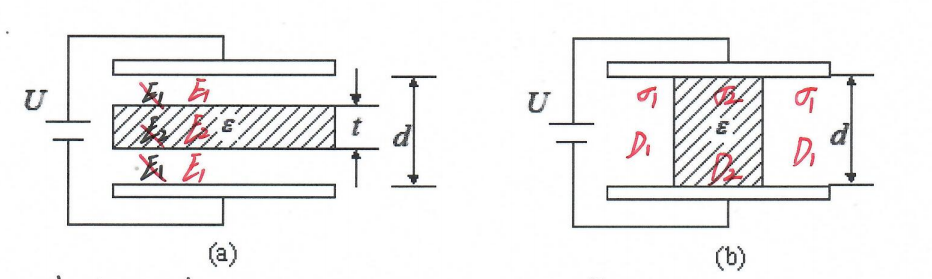
\includegraphics[width=0.8\textwidth]{4.10.png}
\end{center}

\textbf{解答：}

\textbf{(a) 介质板沿电场方向插入（串联模型）}

1. \textbf{电场强度}

介质板厚度为 \(t\)，剩余空气层厚度为 \(d-t\)，两部分电场分别为 \(E_1\)（空气）和 \(E_2\)（介质）。

由电压关系：
\[
U = E_1(d-t) + E_2 t
\]

分界面上电位移法向分量连续（无自由电荷）：
\[
D_1 = D_2 \implies \varepsilon_0 E_1 = \varepsilon E_2
\]

联立解得：
\[
E_1 = \frac{\varepsilon U}{\varepsilon_0 t + \varepsilon(d-t)}, \quad
E_2 = \frac{\varepsilon_0 U}{\varepsilon_0 t + \varepsilon(d-t)}
\]

\vspace{0.5em}
2. \textbf{电荷分布}

极板上的自由电荷面密度由电位移决定：
\[
\sigma = D_1 = \varepsilon_0 E_1 = \frac{\varepsilon_0 \varepsilon U}{\varepsilon_0 t + \varepsilon(d-t)}
\]

介质表面的极化电荷面密度为：
\[
\sigma_p = P = (\varepsilon - \varepsilon_0)E_2 = \frac{(\varepsilon - \varepsilon_0)\varepsilon_0 U}{\varepsilon_0 t + \varepsilon(d-t)}
\]

\vspace{1em}
\textbf{(b) 介质板垂直电场方向插入（并联模型）}

1. \textbf{电场强度}

介质板与空气层并排，极板间距均为 \(d\)，电压均为 \(U\)，因此：
\[
E_1 = E_2 = \frac{U}{d}
\]

\vspace{0.5em}
2. \textbf{电荷分布}

空气部分电位移：
\[
D_1 = \varepsilon_0 E_1 = \frac{\varepsilon_0 U}{d}
\]

介质部分电位移：
\[
D_2 = \varepsilon E_2 = \frac{\varepsilon U}{d}
\]

对应极板上的自由电荷面密度分别为：
\[
\sigma_1 = D_1 = \frac{\varepsilon_0 U}{d}, \quad
\sigma_2 = D_2 = \frac{\varepsilon U}{d}
\]

介质表面的极化电荷面密度为：
\[
\sigma_p = P = (\varepsilon - \varepsilon_0)E_2 = \frac{(\varepsilon - \varepsilon_0)U}{d}
\]

\vspace{1em}

% 第11题
\item 写出下列静电场的边值问题：

\begin{center}
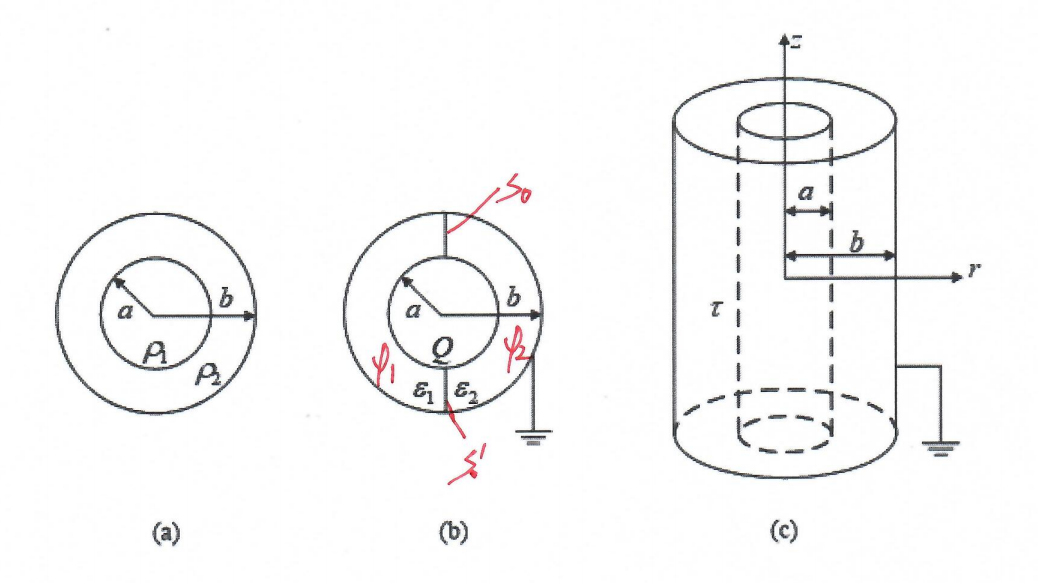
\includegraphics[width=0.8\textwidth]{4.11.png}
\end{center}

\begin{enumerate}
    \item 电荷体密度分别为 \(\rho_1\) 和 \(\rho_2\)，半径分别为 \(a\) 与 \(b\) 的双层同心带电球体，如图(a)所示；
    \item 在两同心导体球壳间，左半部和右半部分别填充介电常数为 \(\varepsilon_1\) 与 \(\varepsilon_2\) 的均匀介质，内球壳带总电荷量为 \(Q\)，外球壳接地，如图(b)所示；
    \item 半径分别为 \(a\) 与 \(b\) 的无限长空心同轴圆柱面导体，内圆柱表面上单位长度的电量为 \(\tau\)，外圆柱面导体接地，如图(c)所示。
\end{enumerate}

\textbf{解答：}

\vspace{0.5em}
(1) 双层同心带电球体（图a）

设电位分布为 \(\varphi(r)\)，根据球对称性，电位仅与径向坐标 \(r\) 有关，分区域写出方程与边界条件：

- 区域1：\(0 \le r < a\)
  \[
  \nabla^2 \varphi_1 = -\frac{\rho_1}{\varepsilon_0}
  \]
- 区域2：\(a < r < b\)
  \[
  \nabla^2 \varphi_2 = -\frac{\rho_2}{\varepsilon_0}
  \]
- 区域3：\(r > b\)
  \[
  \nabla^2 \varphi_3 = 0
  \]

边界条件：
\begin{align*}
& r=0: & & \varphi_1 \text{ 有限} \\
& r=a: & & \varphi_1 = \varphi_2,\quad \varepsilon_0 \frac{d\varphi_1}{dr} = \varepsilon_0 \frac{d\varphi_2}{dr} \\
& r=b: & & \varphi_2 = \varphi_3,\quad \varepsilon_0 \frac{d\varphi_2}{dr} = \varepsilon_0 \frac{d\varphi_3}{dr} \\
& r\to\infty: & & \varphi_3 \to 0
\end{align*}

\vspace{0.5em}
(2) 分区介质同心导体球壳（图b）

设左半区域（\(\varepsilon_1\)）电位为 \(\varphi_1(r)\)，右半区域（\(\varepsilon_2\)）电位为 \(\varphi_2(r)\)，根据球对称性，电位仅与 \(r\) 有关，且两区域电位相等 \(\varphi_1(r)=\varphi_2(r)=\varphi(r)\)。

控制方程（\(a<r<b\)）：
\[
\nabla^2 \varphi = 0
\]

边界条件：
\begin{align*}
& r=a: & & -\left( \varepsilon_1 \int_{\text{左半球}} \frac{\partial \varphi}{\partial r} dS + \varepsilon_2 \int_{\text{右半球}} \frac{\partial \varphi}{\partial r} dS \right) = Q \\
& r=b: & & \varphi = 0 \\
& \theta=\pi/2: & & \varphi_1 = \varphi_2,\quad \varepsilon_1 \frac{\partial \varphi_1}{\partial \theta} = \varepsilon_2 \frac{\partial \varphi_2}{\partial \theta}
\end{align*}

\vspace{0.5em}
(3) 无限长同轴圆柱导体（图c）

设电位分布为 \(\varphi(\rho)\)，根据轴对称性，电位仅与径向坐标 \(\rho\) 有关，区域 \(a<\rho<b\) 内：

控制方程：
\[
\nabla^2 \varphi = 0
\]

边界条件：
\begin{align*}
& \rho=a: & & -2\pi a \varepsilon_0 \frac{d\varphi}{d\rho}\bigg|_{\rho=a} = \tau \\
& \rho=b: & & \varphi = 0
\end{align*}

\vspace{1em}

% 第12题
\item 两个小球半径分别为 \(a=1\,\text{cm}\)，相距为 \(d=20\,\text{cm}\)，位于空气中。
\begin{enumerate}
    \item 若已知 \(\varphi_1\)，\(\varphi_2\)，求 \(q_1\) 和 \(q_2\)；
    \item 若已知 \(\varphi_1\)，\(q_2\)，求 \(q_1\) 和 \(\varphi_2\)；
    \item 问用什么办法使小球1带电荷 \(q_1 = 10^{-8}\,\text{C}\)，小球2不带电荷。
\end{enumerate}

\textbf{解答：}

由于 \(d=20\,\text{cm} \gg a=1\,\text{cm}\)，可近似认为每个小球上的电荷分布均匀，即把它们看作点电荷。设两球电位分别为 \(\varphi_1\) 和 \(\varphi_2\)，由电位叠加原理：
\[
\begin{cases}
\varphi_1 = \frac{1}{4\pi\varepsilon_0} \left( \frac{q_1}{a} + \frac{q_2}{d} \right) \\
\varphi_2 = \frac{1}{4\pi\varepsilon_0} \left( \frac{q_1}{d} + \frac{q_2}{a} \right)
\end{cases}
\]

\vspace{0.5em}
(1) 已知 \(\varphi_1, \varphi_2\)，求 \(q_1, q_2\)。

联立上述方程组，解得：
\[
q_1 = \frac{4\pi\varepsilon_0}{1 - (a/d)^2} \left( a\varphi_1 - \frac{a^2}{d}\varphi_2 \right)
\]
\[
q_2 = \frac{4\pi\varepsilon_0}{1 - (a/d)^2} \left( a\varphi_2 - \frac{a^2}{d}\varphi_1 \right)
\]

\vspace{0.5em}
(2) 已知 \(\varphi_1, q_2\)，求 \(q_1, \varphi_2\)。

由第一个方程解得 \(q_1\)：
\[
q_1 = 4\pi\varepsilon_0 a\varphi_1 - \frac{a}{d}q_2
\]
将 \(q_1\) 代入第二个方程，得 \(\varphi_2\)：
\[
\varphi_2 = \frac{1}{4\pi\varepsilon_0} \left( \frac{4\pi\varepsilon_0 a\varphi_1 - \frac{a}{d}q_2}{d} + \frac{q_2}{a} \right) = \frac{a}{d}\varphi_1 + \frac{q_2}{4\pi\varepsilon_0} \left( \frac{1}{a} - \frac{a}{d^2} \right)
\]

\vspace{0.5em}
(3) 使小球1带电荷 \(q_1=10^{-8}\,\text{C}\)、小球2不带电荷（\(q_2=0\)）的办法。

题目要求：\(\boldsymbol{q_1 = 10^{-8}\,\text{C}}\)（小球1带电），\(\boldsymbol{q_2 = 0}\)（小球2完全不带电）。

直接将小球2接地会使其感应出电荷，无法满足 \(q_2=0\)。正确方法如下：
\begin{itemize}
    \item \textbf{对小球1}：将小球1置于空气中，直接通过充电方式使其带电量为 \(q_1 = 10^{-8}\,\text{C}\)，保持与小球2距离 \(d=20\,\text{cm}\) 不变。
    \item \textbf{对小球2}：将小球2放入一个**接地的闭合金属导体空腔**内部，实现静电屏蔽。
    \item 屏蔽效果：空腔外部电荷 \(q_1\) 的电场无法进入内部，小球2不受任何外电场影响，因此不会产生感应电荷，可保持净电荷 \(q_2=0\)。
\end{itemize}

综上，最终方案：
\textbf{小球1直接充电至 \(q_1=10^{-8}\,\text{C}\)，小球2放入接地金属空腔内实现静电屏蔽，保证 \(q_2=0\)。}

\vspace{1em}

% 第13题
\item 若将某对称的三芯电缆中三个导体相联，测得导体与铅皮间的电容为 \(0.051\,\mu\text{F}\)，若将电缆中的两导体与铅皮相联，它们与另一导体间的电容为 \(0.037\,\mu\text{F}\)，求：
\begin{enumerate}
    \item 电缆的各部分电容；
    \item 每一相的工作电容；
    \item 若在导体 1、2 之间加直流电压 \(100\,\text{V}\)，求导体每单位长度的电荷量。
\end{enumerate}

\begin{center}
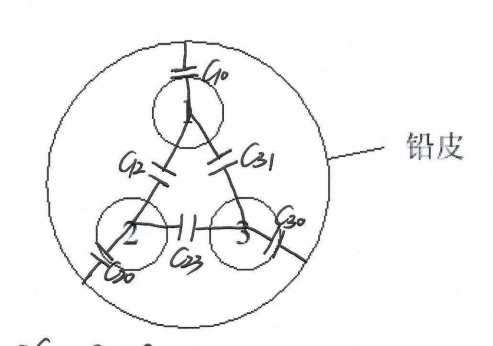
\includegraphics[width=0.6\textwidth]{4.13.png}
\end{center}

\textbf{解答：}

设对称三芯电缆的各部分电容为：
- 导体与铅皮间的电容为 \(C_0\)（每相）
- 导体间的电容为 \(C_1\)（每两相之间）

根据题意，两次测量的电容值可表示为：
1.  三导体相联，与铅皮间的电容：
    \[
    3C_0 = 0.051\,\mu\text{F}
    \]
2.  两导体与铅皮相联，与另一导体间的电容：
    \[
    C_0 + 2C_1 = 0.037\,\mu\text{F}
    \]

\vspace{0.5em}
(1) 求解各部分电容：
由第一个方程得：
\[
C_0 = \frac{0.051}{3} = 0.017\,\mu\text{F}
\]
代入第二个方程：
\[
0.017 + 2C_1 = 0.037 \implies C_1 = \frac{0.037 - 0.017}{2} = 0.01\,\mu\text{F}
\]
因此，电缆的各部分电容为：\(C_0 = 0.017\,\mu\text{F}\)，\(C_1 = 0.01\,\mu\text{F}\)。

\vspace{0.5em}
(2) 每一相的工作电容：
三相对称工作时，每一相的工作电容（导体对地的等效电容）为：
\[
C_\text{ph} = C_0 + 3C_1 = 0.017 + 3 \times 0.01 = 0.047\,\mu\text{F}
\]

\vspace{0.5em}
(3) 导体1、2间加 \(100\,\text{V}\) 电压时的单位长度电荷量：
此时，两导体间的等效电路为：两导体之间通过工作电容 \(C_\text{ph}\) 形成对称结构，可等效为两个串联的 \(C_\text{ph}\) 电容接在 \(100\,\text{V}\) 电压上。
根据电容电荷公式，导体的电荷量为：
\[
Q = \frac{1}{2} C_\text{ph} U
\]
代入数值：
\[
Q = \frac{1}{2} \times 0.047\,\mu\text{F} \times 100\,\text{V} = 2.35\,\mu\text{C}
\]
因此，导体每单位长度的电荷量为 \(2.35\,\mu\text{C}\)。

\vspace{1em}

% 第14题
\item 图(a)所示为镜像法分析静电场分布特性问题。两个点电荷分别位于两种介质中，两种介质的分界面为无限大平面，介电常数分别为 \(\varepsilon_1\) 和 \(\varepsilon_2\)，点电荷 \(q_1\) 与 \(q_2\) 相对于界面为镜像位置，相距为 \(2h\)。用叠加定理分析介质1中的电位 \(\varphi_1\)。当点电荷 \(q_1\) 单独作用时，可按图(b)计算，在图(b)的括号中填入相应的介电常数，此时 \(q_1' = \frac{\varepsilon_1 - \varepsilon_2}{\varepsilon_1 + \varepsilon_2} q_1\)；当点电荷 \(q_2\) 单独作用时，可按图(c)计算，在图(c)的括号中填入相应的介电常数，此时 \(q_2'' = \frac{2\varepsilon_1}{\varepsilon_1 + \varepsilon_2} q_2\)。

\begin{center}
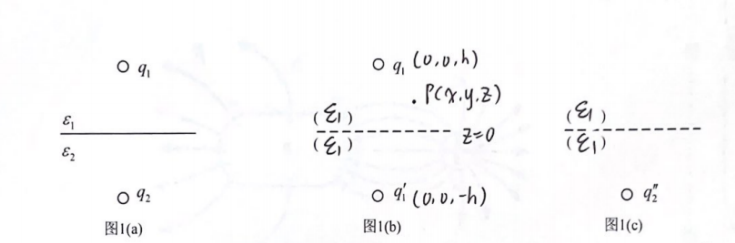
\includegraphics[width=0.8\textwidth]{4.14.png}
\end{center}

\textbf{解答：}

\vspace{0.5em}
(1) 图(b)中，点电荷 \(q_1\) 位于介质1中，为了计算介质1中的电位，需要在介质2中引入镜像电荷 \(q_1'\)。此时，整个空间视为充满介电常数为 \(\varepsilon_1\) 的介质。因此，图(b)的两个括号中均应填入 \(\boxed{\varepsilon_1}\)。
镜像电荷 \(q_1'\) 的大小为：
\[
q_1' = \frac{\varepsilon_1 - \varepsilon_2}{\varepsilon_1 + \varepsilon_2} q_1
\]

\vspace{0.5em}
(2) 图(c)中，点电荷 \(q_2\) 位于介质2中，为了计算介质1中的电位，需要将其等效为位于介质1中的点电荷 \(q_2''\)。此时，整个空间视为充满介电常数为 \(\varepsilon_1\) 的介质。因此，图(c)的括号中应填入 \(\boxed{\varepsilon_1}\)。
等效点电荷 \(q_2''\) 的大小为：
\[
q_2'' = \frac{2\varepsilon_1}{\varepsilon_1 + \varepsilon_2} q_2
\]

\vspace{0.5em}
(3) 介质1中的电位 \(\varphi_1\) 由 \(q_1\) 和 \(q_2\) 共同作用叠加而成：
\[
\varphi_1 = \frac{1}{4\pi\varepsilon_1} \left( \frac{q_1}{r_1} + \frac{q_1'}{r_1'} + \frac{q_2''}{r_2} \right)
\]
其中 \(r_1\) 为场点到 \(q_1\) 的距离，\(r_1'\) 为场点到镜像电荷 \(q_1'\) 的距离，\(r_2\) 为场点到 \(q_2\) 的距离。

\vspace{1em}

% 第15题
\item 试求无限长同轴电容器的单位长度电容。

\begin{center}
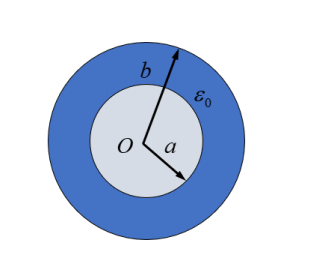
\includegraphics[width=0.4\textwidth]{4.15.png}
\end{center}

\textbf{解答：}

假设内导体的线电荷为 \(\tau\)，根据电荷分布的轴对称性，利用高斯定理求解内外导体间的电场强度。

取半径为 \(r\)、长度为 \(h\) 的同轴圆柱面为高斯面，由高斯定理：
\[
Q = \oint_S \vec{D} \cdot d\vec{S}
\]

高斯面内包围的电荷为 \(Q = \tau h\)，电位移矢量 \(\vec{D} = \varepsilon_0 \vec{E}\)，电场仅沿径向 \(\vec{e}_r\) 方向，因此：
\[
\tau h = \varepsilon_0 E \cdot 2\pi r h
\]

解得电场强度：
\[
\vec{E} = \frac{\tau}{2\pi\varepsilon_0 r} \vec{e}_r
\]

同轴柱面之间的电压为：
\[
U = \int_{a}^{b} \vec{E} \cdot d\vec{r} = \int_{a}^{b} \frac{\tau}{2\pi\varepsilon_0 r} dr = \frac{\tau}{2\pi\varepsilon_0} \ln \frac{b}{a}
\]

根据电容定义，单位长度的电容为：
\[
C = \frac{\tau}{U} = \frac{2\pi\varepsilon_0}{\ln(b/a)}
\]

\end{enumerate}